%%
%% Automatically generated file from DocOnce source
%% (https://github.com/hplgit/doconce/)
%%
%%
% #ifdef PTEX2TEX_EXPLANATION
%%
%% The file follows the ptex2tex extended LaTeX format, see
%% ptex2tex: http://code.google.com/p/ptex2tex/
%%
%% Run
%%      ptex2tex myfile
%% or
%%      doconce ptex2tex myfile
%%
%% to turn myfile.p.tex into an ordinary LaTeX file myfile.tex.
%% (The ptex2tex program: http://code.google.com/p/ptex2tex)
%% Many preprocess options can be added to ptex2tex or doconce ptex2tex
%%
%%      ptex2tex -DMINTED myfile
%%      doconce ptex2tex myfile envir=minted
%%
%% ptex2tex will typeset code environments according to a global or local
%% .ptex2tex.cfg configure file. doconce ptex2tex will typeset code
%% according to options on the command line (just type doconce ptex2tex to
%% see examples). If doconce ptex2tex has envir=minted, it enables the
%% minted style without needing -DMINTED.
% #endif

% #define PREAMBLE

% #ifdef PREAMBLE
%-------------------- begin preamble ----------------------

\documentclass[%
oneside,                 % oneside: electronic viewing, twoside: printing
final,                   % draft: marks overfull hboxes, figures with paths
10pt]{article}

\listfiles               %  print all files needed to compile this document

\usepackage{relsize,makeidx,color,setspace,amsmath,amsfonts,amssymb}
\usepackage[table]{xcolor}
\usepackage{bm,ltablex,microtype}

\usepackage[pdftex]{graphicx}

\usepackage[T1]{fontenc}
%\usepackage[latin1]{inputenc}
\usepackage{ucs}
\usepackage[utf8x]{inputenc}

\usepackage{lmodern}         % Latin Modern fonts derived from Computer Modern

% Hyperlinks in PDF:
\definecolor{linkcolor}{rgb}{0,0,0.4}
\usepackage{hyperref}
\hypersetup{
    breaklinks=true,
    colorlinks=true,
    linkcolor=linkcolor,
    urlcolor=linkcolor,
    citecolor=black,
    filecolor=black,
    %filecolor=blue,
    pdfmenubar=true,
    pdftoolbar=true,
    bookmarksdepth=3   % Uncomment (and tweak) for PDF bookmarks with more levels than the TOC
    }
%\hyperbaseurl{}   % hyperlinks are relative to this root

\setcounter{tocdepth}{2}  % levels in table of contents

% Tricks for having figures close to where they are defined:
% 1. define less restrictive rules for where to put figures
\setcounter{topnumber}{2}
\setcounter{bottomnumber}{2}
\setcounter{totalnumber}{4}
\renewcommand{\topfraction}{0.95}
\renewcommand{\bottomfraction}{0.95}
\renewcommand{\textfraction}{0}
\renewcommand{\floatpagefraction}{0.75}
% floatpagefraction must always be less than topfraction!
% 2. ensure all figures are flushed before next section
\usepackage[section]{placeins}
% 3. enable begin{figure}[H] (often leads to ugly pagebreaks)
%\usepackage{float}\restylefloat{figure}

% prevent orhpans and widows
\clubpenalty = 10000
\widowpenalty = 10000

\newenvironment{doconceexercise}{}{}
\newcounter{doconceexercisecounter}


% ------ header in subexercises ------
%\newcommand{\subex}[1]{\paragraph{#1}}
%\newcommand{\subex}[1]{\par\vspace{1.7mm}\noindent{\bf #1}\ \ }
\makeatletter
% 1.5ex is the spacing above the header, 0.5em the spacing after subex title
\newcommand\subex{\@startsection{paragraph}{4}{\z@}%
                  {1.5ex\@plus1ex \@minus.2ex}%
                  {-0.5em}%
                  {\normalfont\normalsize\bfseries}}
\makeatother


% --- end of standard preamble for documents ---


% insert custom LaTeX commands...

\raggedbottom
\makeindex
\usepackage[totoc]{idxlayout}   % for index in the toc
\usepackage[nottoc]{tocbibind}  % for references/bibliography in the toc

%-------------------- end preamble ----------------------

\begin{document}

% matching end for #ifdef PREAMBLE
% #endif

\newcommand{\exercisesection}[1]{\subsection*{#1}}


% ------------------- main content ----------------------



% --- begin exercise ---
\begin{doconceexercise}
\refstepcounter{doconceexercisecounter}

\exercisesection{Exercise \thedoconceexercisecounter: Dipole in a uniform electric field}


\emph{(Made by: Sigurd Sørlie Rustad)}

\noindent
In this exercise we will take a look at an electric dipole in a uniform electric field. The distance between them is $d$ (see figure under).


\vspace{6mm}

% inline figure
\centerline{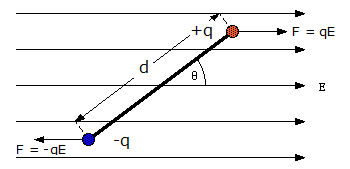
\includegraphics[width=1.0\linewidth]{dipole_efield_fig.png}}

\vspace{6mm}




\subex{a)}
What is the net force on the dipole?


% --- begin solution of exercise ---
\paragraph{Solution.}
$\Sigma \mathbf{F} = 0$

% --- end solution of exercise ---

\subex{b)}
Find the torque in terms of the electric moment $\mathbf{p}$ and the electric field $\mathbf{E}$.

% --- begin hint in exercise ---

\paragraph{Hint.}
The formula for torque is $\bm{\tau} = \mathbf{r}\times\mathbf{F}$, where $\mathbf{r}$ is the the vector going from the point of rotation to where the force $\mathbf{F}$ is applied.

% --- end hint in exercise ---


% --- begin solution of exercise ---
\paragraph{Solution.}
Using the formula for torque and some cross product rules we get
\begin{align}
\bm\tau = \mathbf{r} \times \mathbf{F} = \left(\frac{\mathbf{d}}{2} \times q\mathbf{E}\right) + \left(-\frac{\mathbf{d}}{2} \times (-q\mathbf{E})\right) = q\mathbf{d} \times \mathbf{E} = \mathbf{p}\times\mathbf{E}
\end{align}

% --- end solution of exercise ---

\subex{c)}
For what angles $\theta$ do we have stable and unstable equilibrium? And when do we have maximum torque?


% --- begin solution of exercise ---
\paragraph{Solution.}
Stable equilibrium: $\theta = 0$, Unstable equilibrium: $\theta = \pi$, maximum torque: $\theta = \frac{\pi}{2} \ \ \wedge \ \ \theta = \frac{3\pi}{2}$

% --- end solution of exercise ---

\subex{d)}
Show that for small values of $\theta$ you get a simple harmonic motion. Here you need to use the small angle approximation ($sin(\theta) \approx \theta$) and $\bm\tau = I\bm\alpha$, where $I$ is the moment of inertia and $\bm\alpha$ is the angular acceleration.

% --- begin hint in exercise ---

\paragraph{Hint.}
A simple harmonic oscillator has the differential equation
\begin{equation}
m\frac{d²x}{dt²} = -kx
\end{equation}
Where $m$ and $k$ are constant and $x$ describes the harmonic motion. The solution is
\begin{equation}
x(t) = Acos(\omega t + \phi) \ \ \ \ \omega = \sqrt{\frac{k}{m}}
\end{equation}
$A$ and $\phi$ are constant.

% --- end hint in exercise ---


% --- begin solution of exercise ---
\paragraph{Solution.}
Looking at the torque:
\begin{equation}
\bm\tau = \mathbf{p}\times\mathbf{E} \implies \tau = -|\mathbf{p}||\mathbf{E}|sin(\theta) = I\alpha
\end{equation}
Using the small angle approcimation we get
\begin{equation}
I\alpha \approx -|\mathbf{p}||\mathbf{E}|\theta
\end{equation}
This gives us the differential equation
\begin{equation}
I\frac{d²\theta}{dt²} = -|\mathbf{p}||\mathbf{E}|\theta
\end{equation}
This is an equation for a simple harmonic oscillator.

% --- end solution of exercise ---

\subex{e)}
What is the angular velocity?


% --- begin solution of exercise ---
\paragraph{Solution.}
\begin{equation}
\omega = \sqrt{\frac{|\mathbf{p}||\mathbf{E}|}{I}}
\end{equation}

% --- end solution of exercise ---

\subex{f)}
Find the formula for $\theta$.


% --- begin solution of exercise ---
\paragraph{Solution.}
We are looking for a solution like
\begin{equation}
\theta(t) = Acos(\omega t + \phi)
\end{equation}
In order for energy to be conserved $A = \theta_0$ where $\theta_0$ is the maximum value of $\theta$. $\omega$ is known and $\phi$ depends on the initial conditions, lets say the $\theta$ peaks at $t=0$, then $\phi = 0$. The angle $\theta$ can therefore be described by the equation
\begin{equation}
\theta(t) = \theta_0 cos\left(\sqrt{\frac{|\mathbf{p}||\mathbf{E}|}{I}}t\right)
\end{equation}

% --- end solution of exercise ---

\subex{g)}
Plot the angle over two periods.

% --- begin hint in exercise ---

\paragraph{Hint.}
The formula for moment of inertia for point mass
\begin{equation}
I = \sum_i m_ir_i² 
\end{equation}
$m_i$ is the mass and $r_i$ the distance from the point of rotation to the point mass.

% --- end hint in exercise ---


% --- begin solution of exercise ---
\paragraph{Solution.}
\begin{verbatim}
import numpy as np
import matplotlib.pyplot as plt
import scipy.constants as const
theta0 = (10.0/180)*np.pi   # initial displacement in radians
q = const.e                 # charge on dipole in Coulombs
d = 1e-20                   # distance separating the charges (m)
m = const.m_e               # mass of a single charge (kg)
E = 1e-3                    # magnitude of the electric field
I = 2*m*(d/2)**2            # moment of inertia
p = q*d                     # electric moment
omega = np.sqrt(p*E/I)      # angular frequency
T = 2*np.pi/omega           # period
t = np.linspace(0, 2*T, 2000)  # time interval from t = 0 to t = 2T
theta = theta0*np.cos(omega*t) # solution for Simple harmonic motion
#Plot
plt.plot(t, theta)
plt.title("Simple Harmonic Motion - dipole in an Electric field")
plt.x\label("time (s)")
plt.y\label("angle (radians)")
plt.grid()
plt.show()
\end{verbatim}

% --- end solution of exercise ---

\subex{h)}
Find the numeric solution (do not use small angle approximation) and plot both results over four periods. Use SciPy's odeint package to solve the differential equation. The initial conditions are $q = e$, $d=3\times 10^{-9}$m, $m=3\times 10^{-5}$kg and $E=1000$N/C.


% --- begin solution of exercise ---
\paragraph{Solution.}
\begin{verbatim}
import numpy as np
import matplotlib.pyplot as plt
from scipy.integrate import odeint
theta = np.pi/6         # intial angle of displacement (degres)
q = 1.0e-19             # Charge on dipole in Coulombs
d = 3.0e-9              # distance separating the charges (m)
p = q*d                 # electric moment
m = 3.0e-5              # mass of a single charge (kg)
E = 1000                # magnitude of the electric field
I = 2*m*(d/2)**2        # moment of inertia
omega = np.sqrt(p*E/I)  #angle velocity
T = 2*np.pi/omega       # period
# number of time intervals
N = int(1e4)
# set the times to evaluate
t = np.linspace(0, 4*T, N)
# compute approximate theta values on the time intervals
Approx_Solution = theta*np.cos(omega*np.array(t))
def torque(x0, t, p, I, E):
    dfdt = np.zeros(2)
    dfdt[0] = x0[1]
    dfdt[1] = -p*E*np.sin(x0[0])/I
    return dfdt
# Set the intial condition [initial angle, initial velocity]
x0 = [theta, 0.0]
# numerically solve the real solution using odeint
sol2 = odeint(torque, x0, t, args=(p, I, E))
# Plot the two solutions
plt.plot(t, Approx_Solution)
plt.plot(t, sol2[:, 0])
plt.grid()
plt.x\label("time (s)")
plt.y\label("angle (rads)")
plt.show()
\end{verbatim}

% --- end solution of exercise ---

\subex{i)}
Expand the code over and plot the difference between the numeric and approximate solution over time. Find where the difference between them is above 0.05 rad. Plot red dots over the numeric solution where that is the case.


% --- begin solution of exercise ---
\paragraph{Solution.}
\begin{verbatim}
# compute the difference between approx and actual on intervals
diff = np.abs(Approx_Solution-sol2[:,0])
# Plot the difference vs time
plt.plot(t, diff)
plt.x\label("time (s)")
plt.y\label("Difference")
plt.show()
#finding where the error is bigger than 0.05 rad
index = np.where(diff>0.05)
# Plot the red dots
plt.plot(t, sol2[:,0], \label='numeric solution')
plt.scatter(t[index], sol2[index,0], color='r', \label='error>0.01 rad')
plt.x\label("time (s)")
plt.y\label("angle (rads)")
plt.legend(loc=1)
plt.grid()
plt.show()
\end{verbatim}

% --- end solution of exercise ---

\end{doconceexercise}
% --- end exercise ---


% ------------------- end of main content ---------------

% #ifdef PREAMBLE
\end{document}
% #endif

